\documentclass[a4paper,8pt,openany]{book}
\usepackage[utf8]{inputenc}
\usepackage[french]{babel}
\usepackage[T1]{fontenc}
\usepackage{graphicx}
\usepackage{titlesec}
\usepackage{comment}
\usepackage{amsmath}
\usepackage{amsfonts}

\titleformat{\chapter}[block]
  {\normalfont\Huge\bfseries}% font of number
  {\chaptertitlename\ \thechapter~:}% format of number
  {20pt}% space between number and title
  {\Huge}% font of title

\titlespacing*{\chapter}
  {0pt}%  indent
  {0pt}% space before
  {20pt}% space after
\titlespacing*{\section}
  {0pt}%  indent
  {3.5ex plus 1ex minus .2ex}% space before
  {2.3ex plus .2ex}% space after

\author{Mendy Fatnassi}
\title{Algebre et Arithmetique}

%%%%%%%%%%%%%%%%%%%%%%%%%%%%%%%%%%%%%%	Page	%%%%%%%%%%%%%%%%%%%%%%%%%%%%%%%%%%%%%%%%
\begin{document}
\maketitle
\tableofcontents

\chapter{Vocabulaire & Generalité}

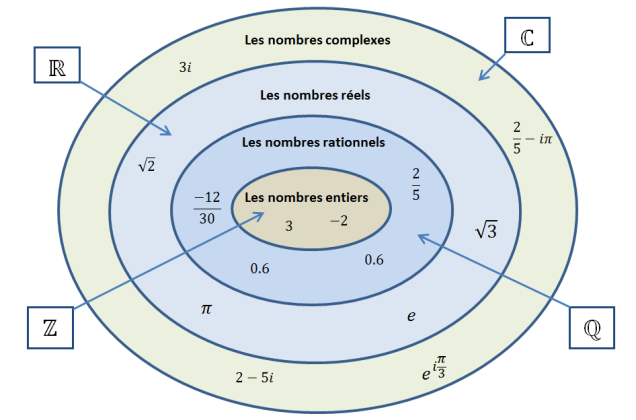
\includegraphics[width=0.60\textwidth,center]{ensembles.png}\\
\\
Et on a N le plus petit ensemble compris dans Z .\\
N est donc l'ensemble des entier positif naturel.\\

\chapter{Arithmetique}

\section{Fraction}
\textbf{Multiplication par un entier} : \\
\\
Si on a un reel k $\in$ R : $k \time \frac{a}{b} \Rightarrows \frac{k.a}{b}$ .\\
\\
\textbf{Multiplication de deux fraction}\\
\\
$\frac{a}{b} \time \frac{c}{d} = \frac{a.c}{b.d}$ \\

\section{Puissances \& Racines}
\\
\underline{Puissances} :\\
\\
$a^x\cdot a^y=a^{x+y}$\\
\\
$\left( \frac{a^x}{a^y} \right)=a^{x-y};$\\
\\
$a^{-x}=\left( \frac{1}{a^n} \right) ;$\\
\\
$(a^x)^y=a^{xy};$\\
\\
$a^x.b^x=(ab)^x;$\\
\\
\underline{Racines} :\\
\\
$\sqrt{a}\times \sqrt{b}=\sqrt{a\times b}$ \\
\\
$ \left( \frac{\sqrt{a}}{\sqrt{b}} \right) =\sqrt{\frac{a}{b}}$ \\
\\
$\sqrt{a^2}=a $ \\




\end{document}